\documentclass[11pt]{article}
\usepackage{graphicx}
\usepackage{hyperref}
\usepackage{natbib}

\setlength{\textwidth}{6.5in}
\setlength{\headheight}{0in}
\setlength{\textheight}{8.0in}
\setlength{\hoffset}{0in}
\setlength{\voffset}{0in}
\setlength{\oddsidemargin}{0in}
\setlength{\evensidemargin}{0in}

\title{Stellar Structure}
  
\author{Michael R. Blanton}


\begin{document}

\maketitle

\abstract{This report describes a simplified solution to the equations
of stellar structure.}

\section{Introduction}
\label{sec:intro}

\section{The Stellar Structure Equations}

We have been told that for a star with energy transport dominated by
radiative diffusion:
\begin{eqnarray}
\frac{\dd{r}}{\dd{m}} &=& \frac{1}{4\pi r^2 \rho} \cr
\frac{\dd{P}}{\dd{m}} &=& -G \frac{m}{4\pi r^4} \cr
\frac{\dd{L}}{\dd{m}} &=& \mathcal{E} \cr
\frac{\dd{T}}{\dd{m}} &=& - \frac{3}{16 \sigma } \frac{\kappa}{T^3}
\frac{L}{(4\pi r^2)^2}
\end{eqnarray}
where $r$ is the radius, $m$ is the mass enclosed within $r$, $L$ is
the luminosity generated within $r$, $P$ is the pressure, $T$ is the
temperature, and $\rho$ is the density. $\mathcal{E}$ is the energy
generated per unit mass and $\kappa$ is the opacity of the
gas. $\sigma$ and $c$ are the Stefan-Boltzman constant and the speed
of light.

The boundary conditions are that $r=0$ and $L=0$ at $m=0$, and that
$P=0$ and $T=0$ at $m=M_\ast$.

We are asked to recast these equations into a form with a minimal
number of unit-full parameters. We can write:
\begin{eqnarray}
\tilde{m} &=& \frac{m}{M_\ast} \cr
\tilde{\rho} &=& \frac{\rho}{\rho_0} \cr
\tilde{r} &=& \frac{r}{R} \cr
\tilde{P} &=& \frac{P}{GM_\ast^2 / R^4} \cr
\tilde{L} &=& \frac{P}{GM_\ast^2 / R^4} \cr
\end{eqnarray}
Where $R = (M_\ast / \rho_0)^{1/3}$. 

\section{Methods}
\label{sec:methods}

This section should contain the problem description, any preliminary
analysis necessary to help set up the computational problem, and how
you did the computation. This section may be fairly long and can be
broken into subsections (as may other sections). You should use your
judgment about how to organize this section for readability.

\subsection{Formulation of the problem}
\label{sec:formulation}

For example, one section might describe how to write the problem in a
mathematically convenient form.

\subsection{Computational methods}
\label{sec:computational}

Another section might describe the specific computational methods.

\section{Results}
\label{sec:results}

This section should contain the results. If appropriate, it should
start with test cases with known solutions or other validation tests
for the methods. Then it should go on to show the results of your
analysis for the more interesting cases.

The discussion in this section is best if it is fairly minimal. ``Just
the facts'' is good place to start. Sometimes it is useful however to
impose some narrative flow; i.e. describe why each case is important
to look at.

It can be difficult to judge what is appropriate to put in the
report. You should begin by being very inclusive regarding the results
you should.

This section should definitely have figures (e.g. Figure
\ref{fig:example}), though they may be appropriate in other sections
too.

\begin{figure}[b!]
\centering
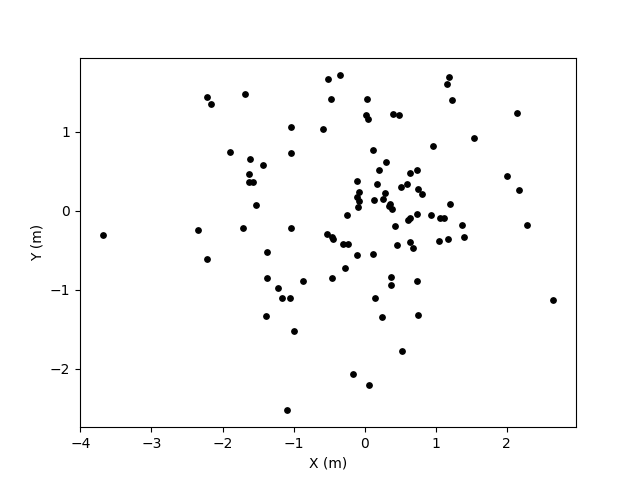
\includegraphics[width=0.95\textwidth]{scatter.png}
\caption{ \label{fig:example} This is just an example. Notice that
  both axes of the figure are labeled, and the units are given.}
\end{figure}
  
\section{Discussion}

The discussion should be where you impose interpretation on the
results. This discussion will have different forms depending on the
goals of the project. What can you conclude about the problem or about
the methods involved? Are you able to reach a conclusion about the
relative merits of different methods? Are these results expected? How
does this work compare with previously determined results? What are
the caveats and limitations of this work?

\bibliographystyle{apj}
\bibliography{example}

\end{document}

 
 
